\chapter{Controlador}

A arquitetura de controle mais utilizada em quadricópteros, possui várias malhas de controles em sua grande maioria em cascata. Onde primeiramente é realizado um controle em relação a posição do veículo e por conseguinte sua orientação. Como a configuração do sentido das hélices do veículo na água é diferente em relação ao ar, diferentes métodos de controle aplicado.

Na Figura \ref{fig:malhacontrole-01} é possível ver a representação gráfica do que está sendo realizado no simulador, onde é possível foram criadas duas grandes malhas correspondentes para cada meio. A explicação da imagem será dada junto ao código, para mostrar como o controle ocorre.

\section{Controle de Posição}

No trecho de código \ref{controle1} é realizado a inicialização do controlador de posição, onde essencialmente são coletados as posições (x, y e z) e o \textit{yaw} de referência, logo após os valores atuais de posição, \textit{yaw} e velocidade x e y são também adquiridos. O controle em z é feito separadamente, então é calculado o erro da posição em x e em y para ser passado para o controlador.


\lstinputlisting[language = Matlab, caption={Aquisição dos valores para realizar o controle de posição},label={controle1},firstnumber=1,linerange={1-15}]{codigos/controlador.m}

\begin{figure}[!htb]
    \centering
    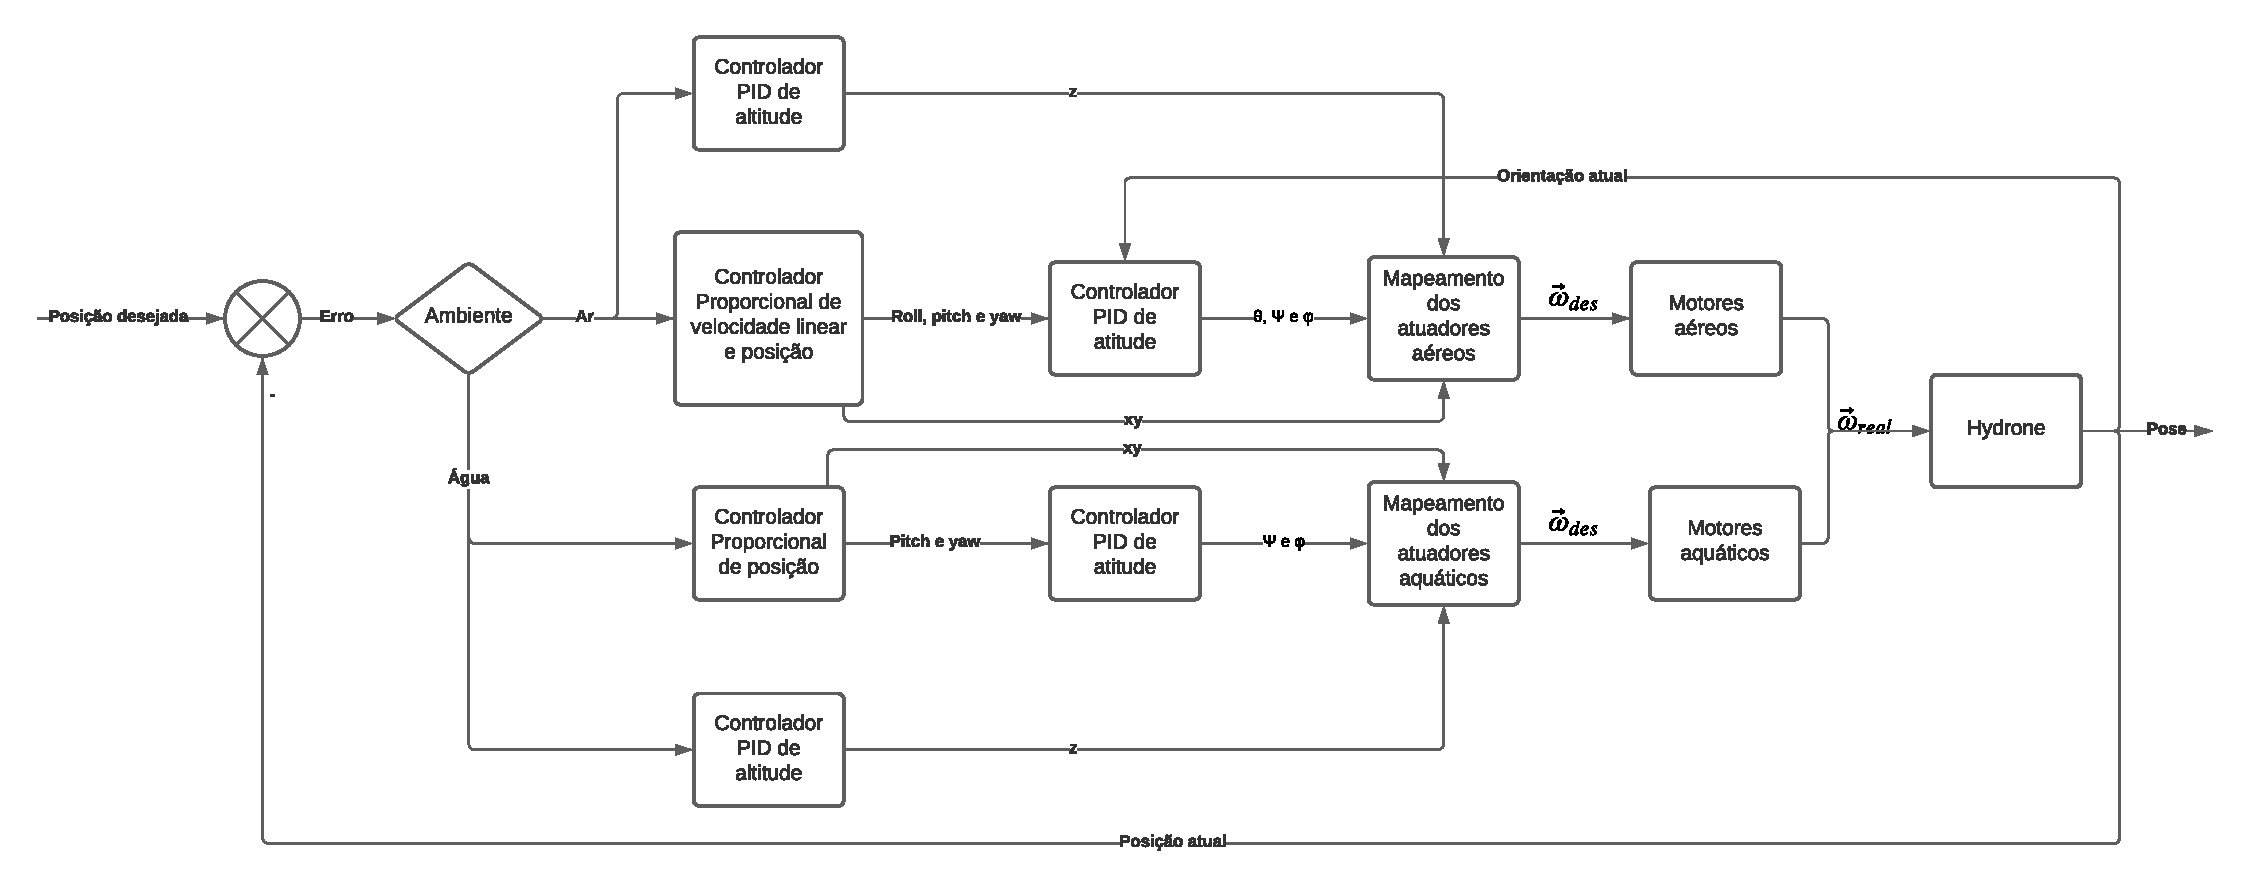
\includegraphics[width=1.4\linewidth, angle =90]{imagens/Controle simulação.pdf}
    \caption{Arquitetura de controle implementada.}
    \label{fig:malhacontrole-01}
\end{figure}

\pagebreak

Seguindo então o diagrama apresentado na Figura \ref{fig:malhacontrole-01} é realizada a verificação do tipo de ambiente, o trecho \ref{controle2} apresenta o controle de posição no ar, onde Kp e Kd são ganhos proporcionais aos erros de posição e velocidade, respectivamente. A variável "R" corresponde a matriz de rotação no eixo z, para mudar os valores de posição e velocidade do referencial local, do veículo, para o global. Por fim, a lei de controle utilizada é apresentada na Equação \ref{controlepos}, sendo ".*", multiplicação de elemento a elemento, gerando valor de referência de \textit{roll} e \textit{pitch} para o ar. Como o controle de x e y no ar é relacionado com a orientação do veículo, o valor de "dv" é zerado.

\lstinputlisting[language = Matlab, caption={Controle de posição no ar},label={controle2},firstnumber=18,linerange={18-36}]{codigos/controlador.m}

\begin{equation}
    \label{controlepos}
    Ang_{ref} =  K_p\begin{bmatrix}
    -1\\
    1
    \end{bmatrix}.*d_p + K_d\begin{bmatrix}
    -1\\
    1
    \end{bmatrix}.*dv
\end{equation}

Caso, o veículo esteja na água, o trecho \ref{controle3} que será utilizado. Na água o controle no plano XY pode ser bastante similar a um veículo diferencial. Primeiramente é calculada a distância euclidiana entre a posição atual e a referência, caso essa distância por maior que um valor de \textit{threshhold} previamente estabelecida o controle será aplicado. Então é coletado e calculado o ângulo entre o alvo e o veículo, tendo seu valor normalizado entre $\pi$ e $-\pi$. Diferentemente do controle no ar, na águam é aplicada uma lei de controle relacionada ao ângulo e a distância até o alvo, podendo ser observado na Equação \ref{equacaoposagua}.

\lstinputlisting[language = Matlab, caption={Controle de posição na água},label={controle3},firstnumber=38,linerange={38-77}]{codigos/controlador.m}

\begin{equation}
    \label{equacaoposagua}
    d_v = k_vd + k_a|\alpha|^2
\end{equation}

\section{Controle de Altitude}

Conforme pode ser visto na Figura \ref{fig:malhacontrole-01} paralelo ao controle de posição é realizado o controle de altitude, o qual está apresentado no trecho \ref{controle4}, onde é utilizada a função "\textit{getU}" que será explicada na Seção \ref{pid}, onde sua grande diferença entre a água e o ar, são os ganhos distintos, determinados no construtor da classe.


\lstinputlisting[language = Matlab, caption={Controle de altitude no ar e na água },label={controle4},firstnumber=80,linerange={80-84}]{codigos/controlador.m}

\section{Controle de Atitude}

Na Figura \ref{fig:malhacontrole-01} após a execução do controlador de posição é realizado o controle de atitude, visto que os valores de referência a serem utilizados é a ação de controle do controlador de posição. No ar, basicamente é aplicado um PID utilizando a "\textit{getU}", podendo ser visto no trecho \ref{controle5}, resultando em 3 sinais de controle, para a correção dos ângulos $\theta$, $\phi$ e $\psi$.

\lstinputlisting[language = Matlab, caption={Controle de atitude no ar},label={controle5},firstnumber=88,linerange={88-100}]{codigos/controlador.m}

Como o Hydrone é subatuado na água, ele não consegue controlar diretamente o $\theta$ do veículo,  conforme é apresentado no trecho \ref{controle6}. Realizando um PID tanto para os ângulos $\phi$ e $\psi$.

\lstinputlisting[language = Matlab, caption={Controle de atitude na água},label={controle6},firstnumber=101,linerange={101-113}]{codigos/controlador.m}

Após todos controles implementados, as contribuições correspondentes ao movimento vertical, longitudinal e de orientação do veículos são manipulador a função "\textit{actuator}", previamente apresentada, resultado nas velocidades desejadas a serem aplicadas nos motores.

\section{Função \textit{getU}(this, rn, yn, dt)}\label{pid}

A função \textit{getU} é a base dos controladores PID's que são utilizados ao longo da simulação, uma explicação sobre alguns detalhes sobre sua implementação são bastante importantes.

Presente como uma função da classe "pid", essa função consiste basicamente em aplicar a lei de controle estabelecida. Inicialmente, conforme pode ser visto no trech \ref{pid1}, são apresentadas três constantes, onde $\gamma$ e $\beta$ são variáveis que ajustam o ganho diretamente, enquanto $\alpha$ corresponde a determinação do tempo do filtro aplicado no cálculo do erro derivativo.


\lstinputlisting[language = Matlab, caption={Parâmetros padrões do algoritmo de controle},label={pid1},firstnumber=50,linerange={50-53}]{codigos/pid.m}

No trecho \ref{pid2} é apresentado o cálculo do erro derivativo, o qual, além do cálculo normal do erro é adicionado um filtro passa-baixa, a fim de eliminar possível valores alta frequência gerados na variação do erro. O valor de $\alpha$ é $0,1$ correspondendo ao tempo de corte do filtro ser $10\%$ do tempo do tempo derivativo.

\lstinputlisting[language = Matlab, caption={Cálculo do erro derivativo com aplicação de um filtro passa-baixa.},label={pid2},firstnumber=64,linerange={64-75}]{codigos/pid.m}

Por fim, como o sistema é todo discretizado, existem diferentes maneiras de se discretizar o PID, no caso, o utilizado foi o modelo do PID ótimo, conforme visto no trecho \ref{pid3}.

\lstinputlisting[language = Matlab, caption={PID ótimo implementado},label={pid3},firstnumber=76,linerange={76-89}]{codigos/pid.m}